\section{Exploring Cloud9}
\label{sec:Motivation}

%\begin{itemize}
%   what c9 can do
%   Tetris
%   how was our development process (team of 3 (2 know git already), cloud9 dashboard, setting up c9 %project (github or bitbucket or without any of them))
%   where do we had problems,
%   our pros and cons for cloud9
%\end{itemize}

%more detailed description of git console
%include Cloud9 Screenshot
%include Tetris Screenshot
After registering for an account on the Cloud9 website or logging in through GitHub or BitBucket\footnote{\url{https://bitbucket.org/}},
the user is led to the Dashboard where he can create new or maintain existing projects as well as access those
shared with him by other members.
Cloud9 supports many languages which amongst others are NodeJS, Javascript, HTML, CSS, Python, Ruby, PHP, C/C++, C\#, Java, and Scala.
While the first two of the mentioned are fully supported in terms of running and debugging other languages are only provided with syntax highlighting.
Once a workspace is created - either from scratch or by cloning from a URL from GitHub or BitBucket -
and the project is launched, the actual editing environment appears (see figure~\ref{fig:cloud9}).
The user interface consists of a navigation pane~\circnum{1} on the left side of the screen and the editing window on the right~\circnum{2}.
At the bottom of the screen is an expandable git command shell~\circnum{3}.

The navigation pane involves various views, accessible through tab icons. The most important one is the project explorer,
which displays all project files in a tree view. Here project files and folders can be edited, deleted or newly created.
Files that cannot be created or edited in Cloud9, such as images, can be dragged and dropped straight from a local hard disk.
Other views include Run \& Debug operations, Server Deployment or text editor settings.
The latter serves the actual coding purposes and supports multiple tabs. Under the hood runs an instance of the Ace
Editor\footnote{\url{http://ace.ajax.org/}}, originally known as Bespin and initially developed by Mozilla Labs,
and provides the user with many of the mandatory text editing features such as syntax highlighting, grouped code indention, and line numbers.
The new release also allows code completion, which has previously only been supported for some commands and
function or variable names that already appeared in one document.
A more detailed view on the Ace editor, its backend components and functionality is provided in section~\ref{sec:ext_editor}.

\begin{figure}
    \centering
    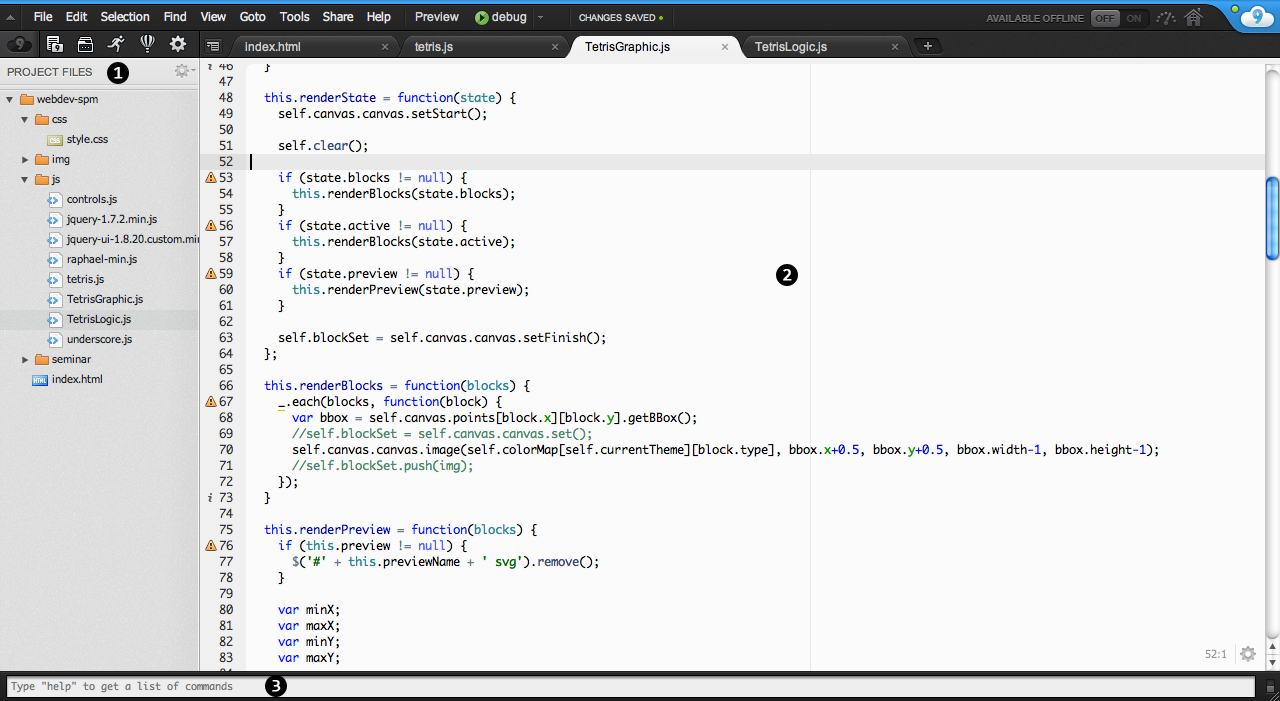
\includegraphics[width=0.9\textwidth]{images/cloud9.png}
    \caption{The Cloud9 workspace view.}
    \label{fig:cloud9}
\end{figure}

\subsection{Developing Tetris}
\label{sec:tetris}
There is not much to say about Tetris, one of the world's most famous computer games. Single objects composed out of four
squares, that fall from the top border of the rectangular playing field, need to be arranged to form complete,
horizontal lines at the bottom of the field.
Our Javascript based implementation offers two players to battle each other with the use of a key shared keyboard.
Players score by dropping objects and generating unbroken lines. Accomplishing more than one line at once will
add the corresponding number of lines to the opponent player's field.
The first player running out of space for new spawning objects loses.
We duplicated the shapes of the original game and included six different levels.
Each level upgrade results in a higher score for each dropped object and cleared line as well as in a higher falling speed of the objects.

%include workflow illustration
Apart from designing the elements of the graphical user interface, which required the use of image processing software,
we were able to accomplish our implementation entirely in a web browser.
However, our development process still did not happen as would be desirable.
Figure ~\ref{fig:workflow} illustrates our development workflow of Tetris.

As seen on the right, debugging still requires the use of additional tools such as Firebug.
Even though Javascript projects are provided with a built in debugging feature,
holding a running program at a breakpoint not only influences the program itself but also the Cloud9 application,
which means that while in hold state no code editing is possible in Cloud9.
While using Firebug or Google's Developer Tools resolves this issue, hot code replacement still remains a desirable
feature to achieve the ``immediate connection'' we previously mentioned.
Up until now a reload of the to be debugged program has to do. Same applies to designing the graphical user interface of
an application.
An integrated Firebug like solution for manipulating and storing a HTML/CSS design would be very desirable
here and critically increase the development experience.

We stored our code in a GitHub repository, which can be pulled from and pushed to by Cloud9's built-in git functionality.
However, the git command shell only comes with a rudimentary support of what git actually has to offer.
Even though it understands the entire range of git commands, suggestions are only made for a small selection.
As one of our team members has not been familiar with git a more sophisticated implementation of this feature would have
resulted in a much more comfortable learning process. Keyword or paragraph highlighting, e.g. added/deleted chunks,
is also missing. What really disrupted a fluent workflow is, however, the fact that the console has to be activated and
expanded every time we want to use it.
Further the console supports no interactive mode, which results in displaying all the output at once and missing possibilities to execute interavtive commands.
In combination with the lack of mentioned features, using an external command shell is more powerful and comfortable.
Cloud9 misses the chance of creating an enjoyable programming experience by harmoniously integrating git functionality into the graphical user interface.

In addition to the described obstacles that prevent
a fluent development workflow, Cloud9 does not seem to run very stable and reliable yet.
During development we run into many situations where files did not load in the editor, changes could not be saved or
duplicate files showed up in the project explorer. Often, in order to clear those situations we had to refresh the page,
i.e. restart the IDE, which also leaves space for improvements.

\begin{figure}
    \centering
    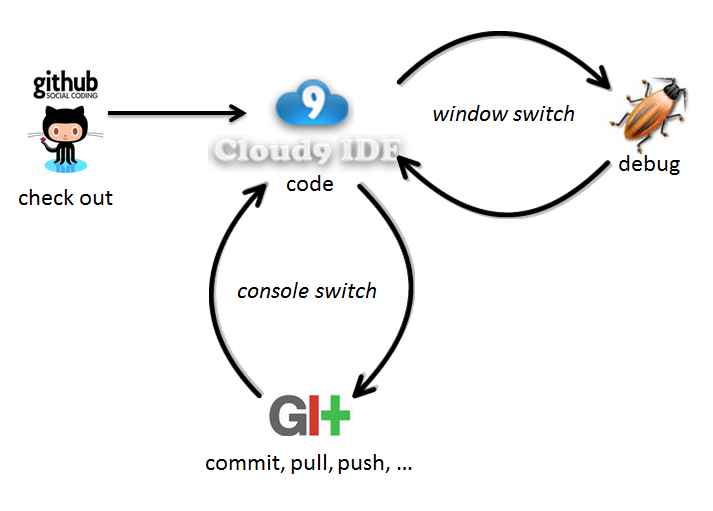
\includegraphics[width=0.5\textwidth]{images/workflow.png}
    \caption{Our development workflow.}
    \label{fig:workflow}
\end{figure}

\subsection{Cloud9 Alternatives}
%list of other tools --> dart, Jens' list
%what other IDEs were on the list
Apart from Cloud9 we considered various other online based development environments or languages as the base for our experiment.
From a selection including Lively Kernel~\cite{Ingalls2008LKS},
Dart\footnote{\url{http://code.google.com/p/dart/}},
or Google's AppInventor~\cite{wolber2011app} just to name a few,
we especially looked into Dart.

We built a little Memory application to evaluate the capabilities of this new web programming language.
Even though we certainly would have enjoyed playing around with it in a bigger project,
development is actually done offline in an Eclipse based editor. Google provides a little online text editor, which,
however, only purposes some coding experiment of the Dart language and is not suitable for serious application development
as fundamental features such as project maintenance are missing. The only way of extending the Dart experience therefore
would have been creating an IDE in the first place, which we considered to be exceeding the effort of what could reasonably
be done within a single semester.
Cloud9 in return appears to have already got over and done with these first steps that
Google is still facing. It gives an impression that is familiar to other known desktop IDEs and left us various options
for possible extensions which finally let us arrive at the decision to give preference to Cloud9.